\begin{frame}{Projection and Parametrization on arbitrary quads}
\begin{overlayarea}{\textwidth}{.15 \textheight}
\begin{enumerate}
\item<1-> find least squares plane approximating quad
\item<2-> projection of datapoint onto plane
\item<3-> find corresponding parameters $\left[u,v\right] \in \left[0,1\right]^2$
\end{enumerate}
\end{overlayarea}
\begin{overlayarea}{\textwidth}{.85 \textheight}
\only<1>{
\begin{columns}
\column{.3\textwidth}
\begin{figure}
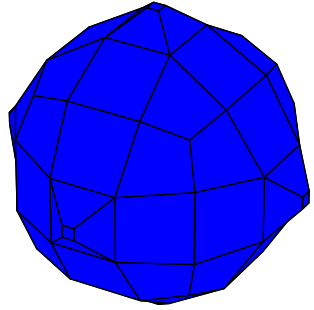
\includegraphics[width = \textwidth]{Pictures/BackupSlidesProjection/nonPlaneQuads.png}
\caption{DC sphere}
\end{figure}
\column{.3\textwidth}
\begin{figure}
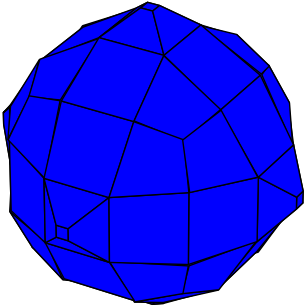
\includegraphics[width = \textwidth]{Pictures/BackupSlidesProjection/withPlaneQuads.png}
\caption{with plane quads}
\end{figure}
\end{columns}
}
\begin{columns}
\column{.35\textwidth}

\begin{overlayarea}{\textwidth}{\textheight}
\begin{figure}
\only<2-3>{
\tdplotsetmaincoords{60}{110}
\begin{tikzpicture}[scale = 1.5,tdplot_main_coords]
\coordinate (O) at (-1,-1,0);
\coordinate[dot] (A) at (0,0,0);
\coordinate[dot] (B) at (1,0,0);
\coordinate[dot] (C) at (1.2,1.5,0);
\coordinate[dot] (D) at (0,1,0);
\coordinate (P1) at (.5,.4,1);
\coordinate (P2) at (1,1,1);
\coordinate (Q1) at (.5,.4,0);
\coordinate (Q2) at (1,1,0);

\draw[thick,->] (O) -- ($(O)+(.5,0,0)$) node[anchor=north east]{$x$};
\draw[thick,->] (O) -- ($(O)+(0,.5,0)$) node[anchor=north west]{$y$};
\draw[thick,->] (O) -- ($(O)+(0,0,.5)$) node[anchor=south]{$z$};

\draw[thick] (A) -- (B) -- (C) -- (D) -- (A);

\only<2-3>{
\draw (P1) node[thick,cross,red,label = {$P_1$}] {};
\draw[red,dashed] (P1) -- (Q1);
\draw (Q1) node[thick,cross,red] {};
}
\only<3>{
\draw (P2) node[thick,cross,red,label = {$P_2$}] {};
\draw[red,dashed] (P2) -- (Q2);
\draw (Q2) node[thick,cross,red] {};
\draw[black,dashed] (B) -- (D);
}
\draw (A) node[label = left:{$A$}]{};
\draw (B) node[label = left:{$B$}]{};
\draw (C) node[label = right:{$C$}]{};
\draw (D) node[label = right:{$D$}]{};
\end{tikzpicture}
}
\end{figure}
\end{overlayarea}

\column{.5\textwidth}
\begin{overlayarea}{\textwidth}{\textheight}
\only<2>{
\begin{block}{Coordinate transformation}
system with basis
\begin{equation*}
B_{BAD} = \left(
\begin{array}{ccc}
\vec{n} & \vec{AB} & \vec{AD}
\end{array}
\right)
\end{equation*}
yields
\begin{equation*}
\left(B_{BAD}\right)^{-1} P_1
=
\left(
\begin{array}{ccc}
d&u&v
\end{array}
\right)^T
\end{equation*}
\end{block}
}
\only<3>{
\begin{block}{Problem:}
\begin{itemize}
\item[\textcolor{green}{\Checkmark}] for $P_1$: $\left(u,v\right) = \left(0.5,0.4\right)$
\item[\textcolor{red}{\XSolidBrush}] for $P_2$: $\left(u,v\right) = \left(1,1\right)$
\end{itemize}
\end{block}

\begin{block}{Solution:}
\begin{enumerate}
\item if we get $u+v > 1$
\item use $B_{BCD}$ instead of $B_{BAD}$
\item set $u=1-u$, $v=1-v$
\end{enumerate}
\end{block}

}
\end{overlayarea}
\end{columns}
\end{overlayarea}
\end{frame}
